\subsection{Workshop}
\label{workshops}

Tjora (2012) påpeker at valg av metode for datagenerering må reflektere hva man faktisk ønsker å finne ut, og at effektivitet bør vektlegges. “Datagenereringen må kunne frambringe mest mulig relevant og pålitelig informasjon uten unødig bruk av forskeres og deltakeres tid og ressurser”.
I tråd med \ref{chp: medvirkning}, ønsket vi en brukersentrert designprosess, hvor brukerene medvirket gjennom en \emph{deltagende design workshop}.
En slik workshop åpner for at utviklere, bedriftsrepresentanter og brukere kan jobbe sammen for å avdekke utfordringer og løsninger på en svært produktiv måte. Dette vil være mest effektivt tidlig i designprosessen, da idèer ikke hemmes av eksisterende kode eller annen infrastruktur (Gaffney, 1999).

\subsubsection{Kontekst}
Vi gjennomførte to workshoper over to dager. Disse ble holdt på NSEP brukbarhetslab (Norsk senter for elektronisk pasientjournal) ved St. Olavs Hospital. Brukbarhetslaben er bygget for å kunne observere og teste mobile helsetjenester \cite{NSEP}.
Som Alsos og Dahl (2008) beskriver, vil sykehus ofte ha strenge restriksjoner mot å tillate eksperimentelle forsøk, da slike forsøk kan ha en påtrengende effekt på det pågående arbeidet. I tillegg kan opptak av observasjoner være forbudt, da pasientinformasjon er konfidensielt. Ved testing i brukbarhetslab kan man fokusere på relevante bruksområder, og kontrollere faktorer irrelevante for evaluering av løsningen \cite{Alsos08}. På grunn av tidsbegrensning var det derfor naturlig å benytte brukbarhetslaben som testmiljø.   


\subsubsection{Artefakter}
\begin{figure}[H]
	\centering
	\begin{subfigure}[b]{0.25\textwidth}
		\centering
		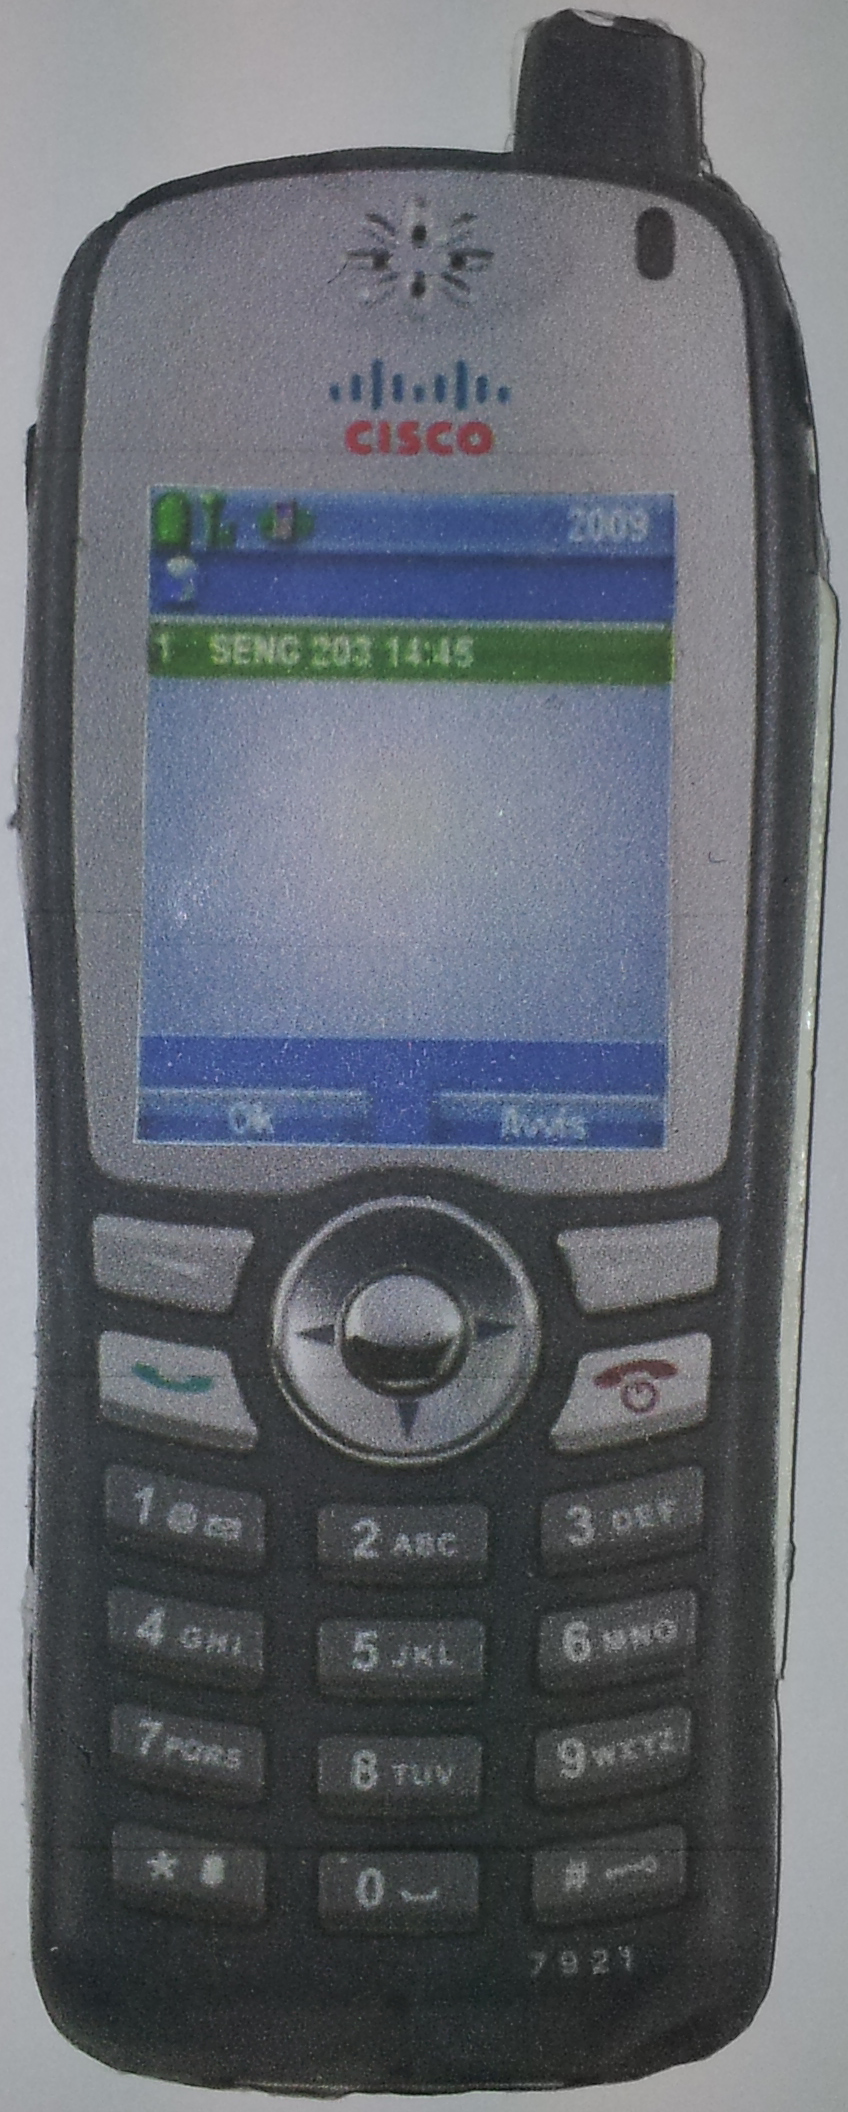
\includegraphics[scale=0.07]{mock-up_Telefon.jpg}
		\caption{Mock-up av telefon}
		\label{mock-up_Telefon}
	\end{subfigure}
	\begin{subfigure}[b]{0.35\textwidth}
		\centering
		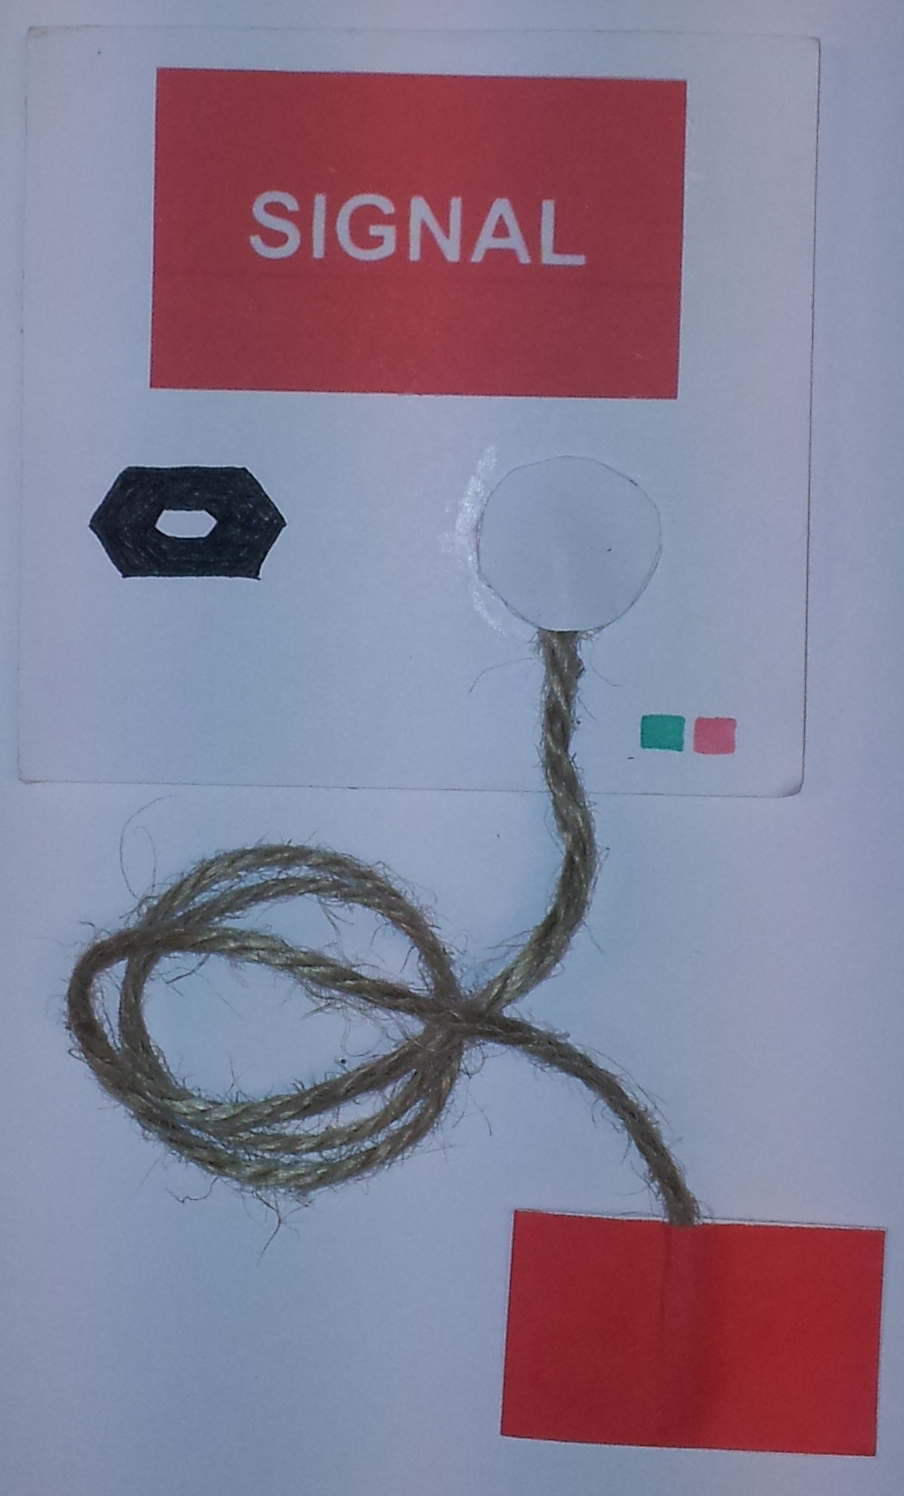
\includegraphics[scale=0.07]{mock-up_PasientPanel.jpg}
		\caption{Mock-up av anropspanelet}
		\label{mock-up_PasientPanel}
	\end{subfigure}
	\begin{subfigure}[b]{0.35\textwidth}
		\centering
		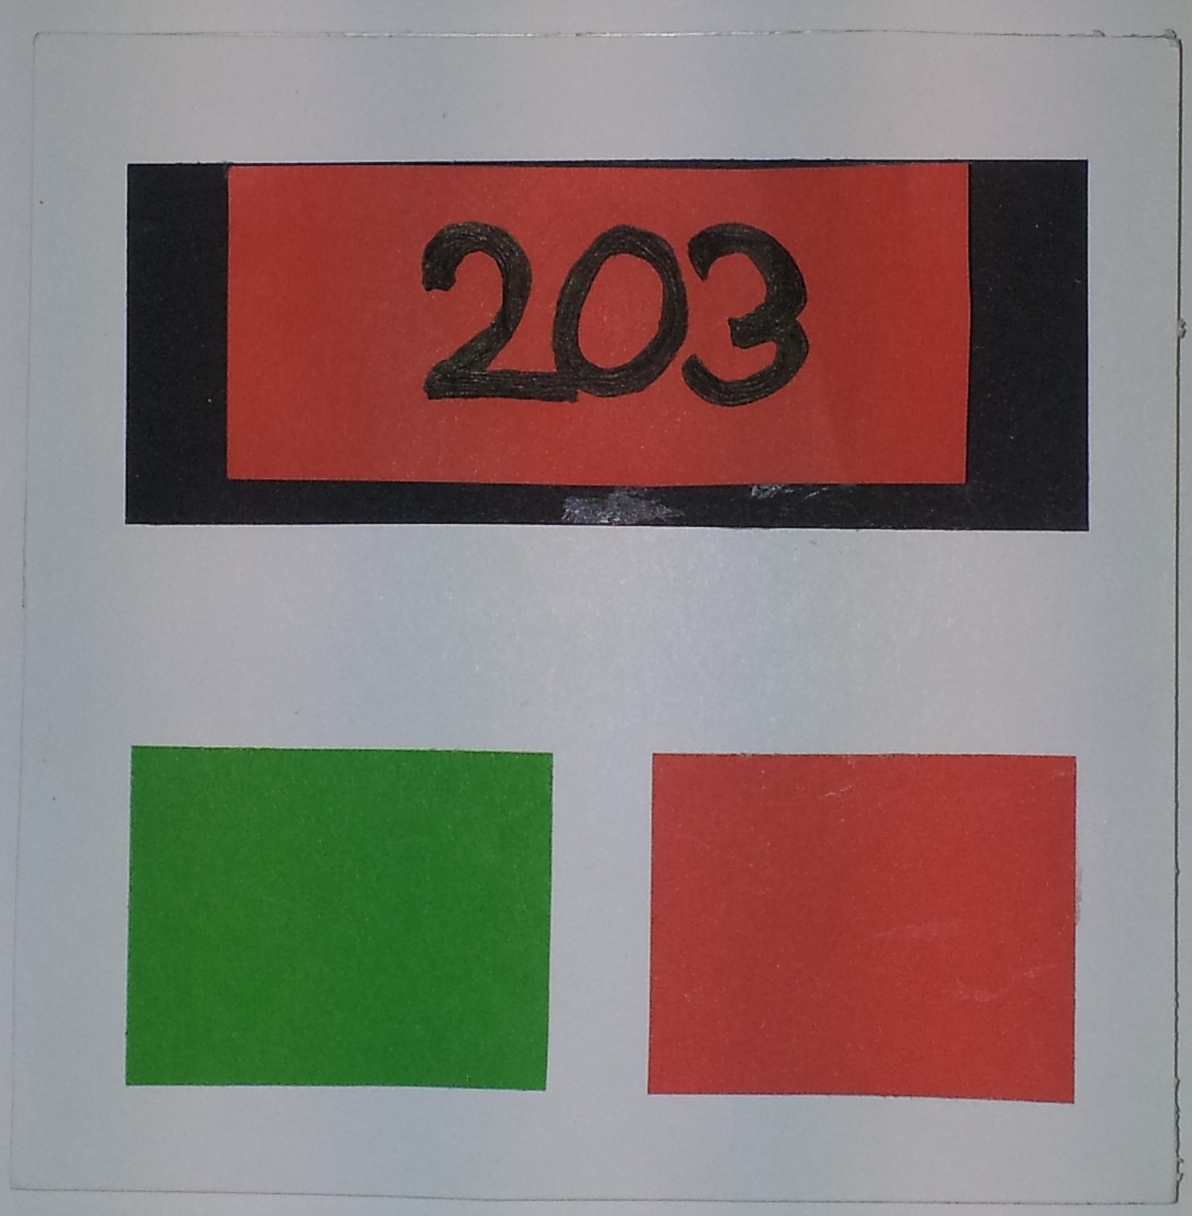
\includegraphics[scale=0.07]{mock-up_RomPanel.jpg}
		\caption{Mock-up av rompanelet}
		\label{mock-up_RomPanel}
	\end{subfigure}
\end{figure}

\begin{figure}[H]
\centering
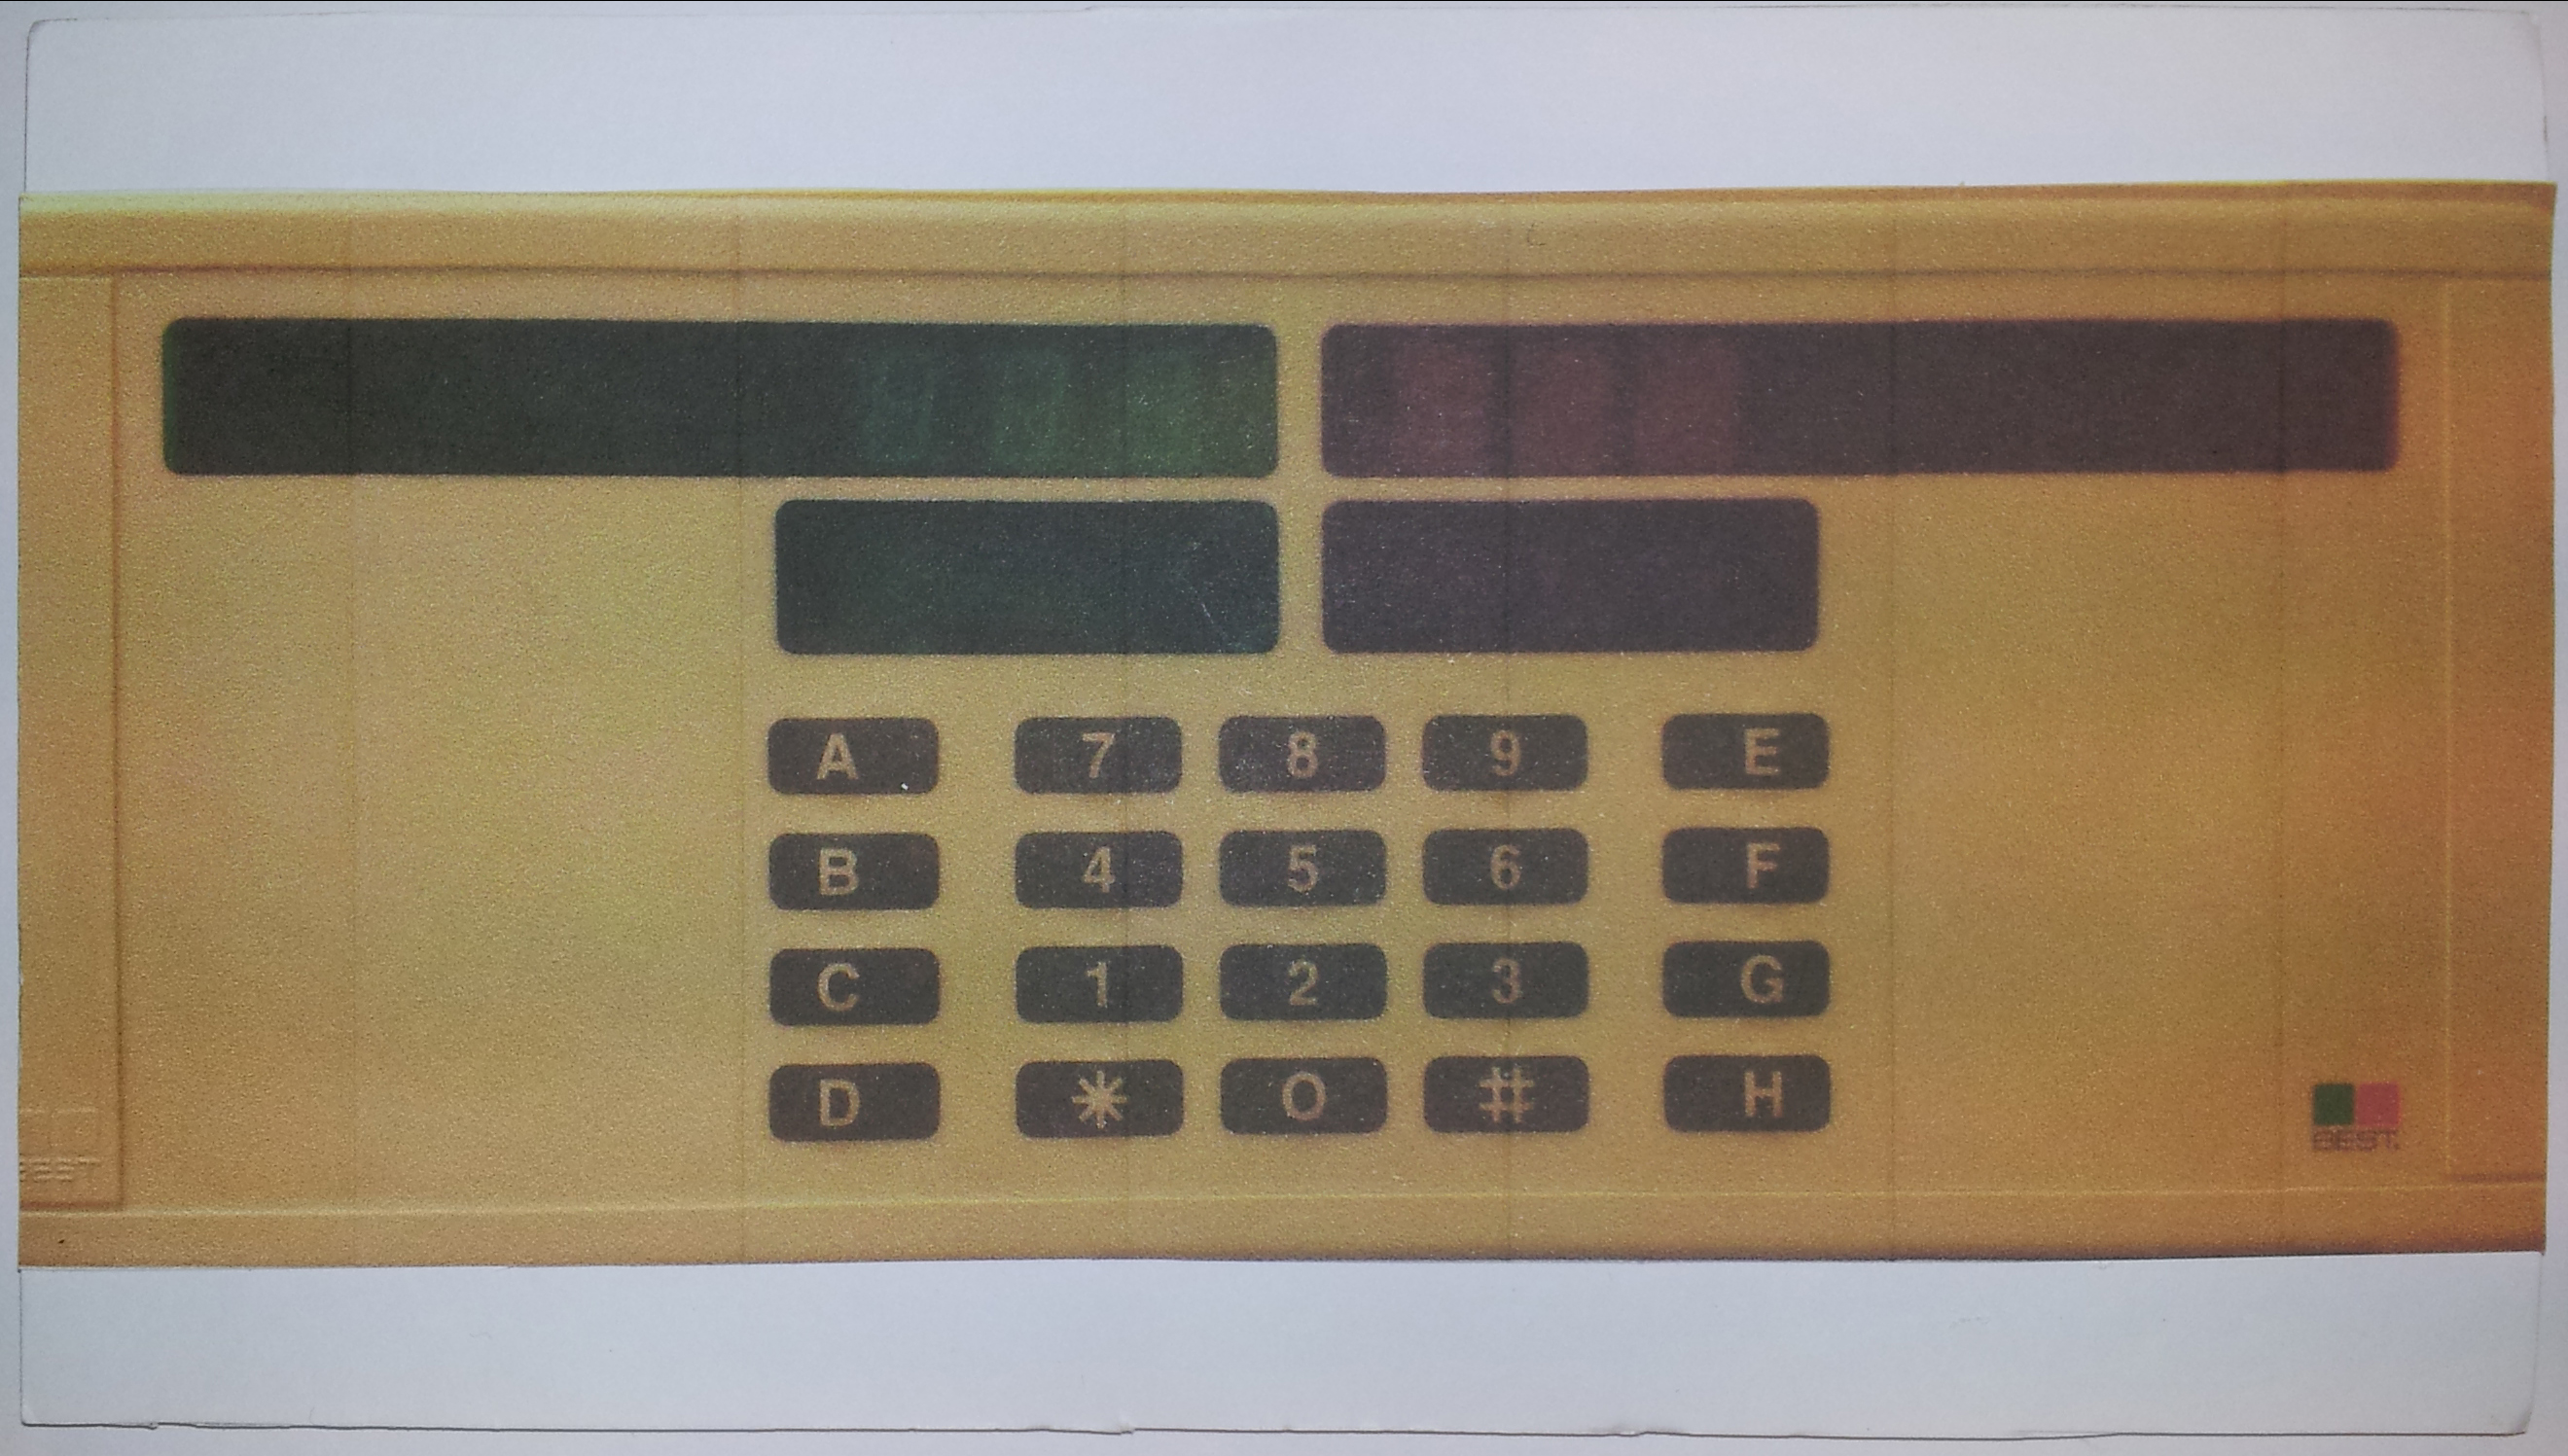
\includegraphics[scale=0.07]{mock-up_VaktPanel.jpg}
\caption{Mock-up av vaktromsapparatet}
\label{mock-up_VaktPanel}
\end{figure}

\subsubsection{Scenarioer}
Som beskrevet av Svanæs og Seland (2004), er rollespill med bruk av lavnivå-protoype en god måte å få brukere og utviklere "opp av stolen", og gjør det mulig å utforske designkonsepter med brukere i en tidlig fase. Scenario-basert design, belyst av Bardram (2000), er nyttig i situasjoner hvor man ikke har en detaljert oppfattelse av nøyaktig hvilke arbeidsaktiviteter som skal støttes, og på hvilken måte. Denne designprosessen har to karakteristikker, (1) man ønsker å re-designe de eksisterende måtene å gjøre ting på for å forstå hvordan ting kan gjøres annerledes ved hjelp av et datasystem. Dette starter ofte ved at man undersøker problemene og fordelene med det eksisterende systemet. (2) Deretter starter den kreative prosessen, hvor designeren, med sin tekniske erfaring, og brukeren, med sin arbeids- og organisasjonserfaring, sammen kommer opp med nye ideer. Relevante spørsmål man bør stille seg i en slik prosess er; er disse ideene nyttige? Og hvilke arbeidsaktiviteter støtter de, og hvilke forstyrrer de? Bruk av scenarioer er dermed nyttig fordi de støtter det kreative samspillet mellom designer og bruker, og de besvarer spørsmål om nyttigheten til systemet i forhold til arbeidsrutinene i en organisasjon. Det Bardram (2000)\nocite{Bardram00} kaller arbeidsaktivitets-scenarioer, er scenarioer som prøver å få en klarhet i det arbeidet vi ønsker å designe for. 
I tråd med det Bardram (2000) skriver, var det ønskelig å bruke to sett med scenarioer, ett hvor det eksisterende systemet og arbeidspraksis ble brukt, og ett hvor vi testet våre ideer i form av en prototype, for å skape en kreativ prosess for videre forslag og innspill fra deltagerne. Det ble tatt utgangspunkt i scenarioer og pasientbeskrivelser fra Selseth (2012)\nocite{Selseth12}, med noen modifikasjoner for å gjøre de relevante til våre forskningsspørsmål. Scenarioene i sin helhet er vedlagt som en del av tillegg B, og pasientbeskrivelsene er vedlagt i tillegg C.

%\begin{adjustbox}{with=\textwith, hight=\texthight}
\begin{table}[H]
%\small
\caption{Overordnet plan for dagen}
%\centering
\begin{tabular}{l|l|l|l|l}
\hline
\textbf{\begin{tabular}[x]{@{}c@{}}Del av\\workshop\end{tabular}} & \textbf{Beskrivelse} & \textbf{Hvor} & \textbf{Tidspunkt} & \textbf{Varighet}\\
\hline
Steg 1 & Informasjon & \begin{tabular}[x]{@{}c@{}}Rundt bord\\/i gangen\end{tabular} & 13:00-13:15 & 15min\\
\hline
Steg 2 & Fokusgruppe med scenarioer & \begin{tabular}[x]{@{}c@{}}Rundt bord\\/i gangen\end{tabular} & 13:15-13:45 & 30min\\
\hline
& \textbf{Pause} & & 13:45-13.50 & 5min\\
\hline
Steg 3 &\begin{tabular}[x]{@{}c@{}} Scenarioer med rollespill\\- uten prototype\end{tabular} & Inne på sengerom & 13:50-14:25 & 35min\\
\hline
Steg 4 &\begin{tabular}[x]{@{}c@{}}Scenarioer med rollespill\\- med prototype\end{tabular} & Inne på sengerom & 14:25-15:00 & 35min\\
\hline
& \textbf{Pause} & & 15:00-15:15 & 15min\\
\hline
Steg 5 & Fokusgruppe/oppsummering & \begin{tabular}[x]{@{}c@{}}Rundt bord\\/i gangen\end{tabular} & 15:15-16:00 & 45min
\end{tabular}
\label{Plan}
\end{table}
%\end{adjustbox} 

\noindent
Som vist i tabell \ref{Plan}, ble scenarioene delt i tre deler. I steg 2 forsøkte vi å avdekke generelle likheter og ulikheter mellom avdelingene, knyttet til ansvarsfordeling og situasjoner hvor det kunne være ønskelig å være utilgjengelig. Dette ble gjort gjennom fokusgruppediskusjon, hvor deltagerene ble presentert generelle scenarioer. I steg 3 ønsket vi å avdekke problemer og fordeler med det eksisterende systemet og arbeidspraksis. Her fikk deltagerene spille ut to scenarioer, med bruk av artefakter som skulle representere det eksisterende systemet. I steg 4 ønsket vi å teste vår foreslåtte løsning. Deltagerene ble derfor bedt om å spille ut de samme scenarioene med bruk av den nye løsningen. Utførelse av workshopene vil bli beskrevet nærmere i \ref{deltagere}.

\subsubsection{Fokusgruppe}
Fokusgrupper kan være en effektiv form for datagenerering fordi man utvikler intervjudata fra flere informanter samtidig \cite{Tjora}. Slike grupper fremkaller ofte spontane reaksjoner og ideer \cite{Nielsen97}, og informantene kan stimulere hverandre, og dermed få frem mange aspekter av informantenes opplevelser av fenomener de alle kjenner til. Erfaringen fra fokusgruppen kan være kilde til nye tanker og refleksjoner \cite{Tjora}. Bruk av fokusgrupper har ikke nødvendigvis til hensikt å vurdere brukergrensesnitt og brukbarhet, men heller å avklare hva brukerene ønsker av systemet. En av utfordringene er derimot at deltagerene kan tro at de ønsker noe, mens de kanskje \emph{trenger} noe helt annet. Derfor er konkrete eksempler, eksempelvis bruk av prototype og scenarioer, en god måte å måle eller observere hvordan brukerene faktisk bruker noe \cite{Nielsen97}.
For å styre ordet og sørge for at alle får sagt de ønsker, brukes moderatorer. Disse vil også formulere spørsmål for å sette i gang diskusjoner, og eventuelle oppfølgingsspørsmål \cite{Tjora}. 

\noindent
Første dag var Veronica moderator og Monika assisterende moderator, og motsatt dag to. I tillegg deltok Joakim Klemets som assisterende moderator begge dager. De assisterende moderatorene stilte utfyllende spørsmål ved behov og ønske. Da det ble tatt videoopptak av workshopene var det ikke nødvendig at de assisterende moderatorerene dokumenterte sesjonene. 

\subsubsection{Videoopptak}
Videoopptak har ifølge Tjora (2012) en vesentlig fordel når det kommer til å gjøre detaljert analyse av handling og samgandling. Samtidig er videodata mer krevende å håndtere enn for eksempel kun lydopptak. I tillegg til det praktiske og etiske rundt bruk av videoopptak og at det genereres store mengder data på denne måten, kan de som filmes endre oppførsel som resultat av filmingen, og dermed påvirke forskningsresultatene. Videoopptak brukes ofte for å få med alle detaljer i samhandligen, og gir en ikke-tolket gjengivelse av situasjonen. Bruk av video vil i så måte gi et større fokus på detaljer. En blir oppmerksom på hvir mye detaljene betyr i sammenhengen, og det kan bli vanskelig å trekke ut ekstrakter til en analyse. 
Videostøttede observasjoner gjør det også mulig å gjøre analysen sammen med andre. Som observtør er man ofte så dypt innvolvert i situasjonen, og feltnotatene vil bli en i noen grad fortolket beskrivelse. Dette gjør det vanskelig for veiledere og kolleger å bidra med analysen og komme med innspill på hvordan situasjonene kan tolkes. 
Bruk av video kan også by på utfordringer, som sviktende teknisk utstyr, uheldig plassering av kameraer og dårlig lyd.

\noindent
Bruk av videoopptak ble et naturlig valg da denne løsningen ble foreslått til oss av veileder og professor, og disse hadde gode erfaringer med dette fra tidligere. Vi oppdaget i midlertid at dette var en fordel når vi var to som skulle gå gjennom opptakene i ettertid, samt muligheten til å enkelt kunne identifisere hvem som sa hva under fokusgruppediskusjonene var en stor fordel. 
Vi var heldige å fikk bruke brukbarhetslaberatoriet til NSEP hvor det allerede er montert bevegelige kameraer og mikrofoner i alle rom, samt at tilstederværende senioringeniør hadde ansvar for opptakene. Dette var med på å sikre oss gode opptak som lettet arbeidet med analysen i ettertid.


\subsubsection{Deltagere og utførelse}
\label{deltagere}
Det ble i forkant av workshopene sendt mail til de ansvarlige for sykepleierstudentene, med den intensjon å rekruttere studenter gjennom disse. Da påmeldingen gikk sent, ble det behov for å ringe og besøke de ulike sengetunene på St. Olavs Hospital, for å komme i direkte kontakt med studentene. 
Det ble arrangert to like workshoper, WS1 og WS2, med totalt 9 deltagere, se tabell \ref{DeltagereWS}. Alle deltagere og avdelinger er anonymisert, og kolonnen \emph{Notasjon} er brukt for å knytte resultatene til de aktuelle deltagerene. Alle deltagerene var andreårs sykepleierstudenter ved HiST (Høyskolen i Sør-Trøndelag). Da vi hadde behov for alle de påmeldte, var vi ikke i en posisjon hvor vi kunne velge ut deltagere for å få en viss gruppesammensetting. Det at vi kun hadde tilgang til studenter, og ikke arbeidende sykepleiere, medførte at deltagerene hadde begrenset erfaring med systemet, og man kan stille spørsmål til hvorvidt utvalget var representativt. Da studentene er aktuelle fremtidige brukere av systemet vi ønsket å teste, anså vi likevel workshopene som nyttige.

\begin{table}[H]
\begin{tabular}{ |l|l|l|l| }
\hline
\multicolumn{4}{ |c| }{Deltagere ved workshoper} \\
\hline
WS & Deltagere & Avdeling & Notasjon \\ \hline
\multirow{4}{*}{WS1} & S1 & A1 & S1-A1 \\
 & S2 & A2 & S2-A2 \\
 & S3 & A3 & S3-A3 \\
 & S4 & A3 & S4-A3 \\ \hline
\multirow{5}{*}{WS2} & S5 & A3 & S5-A3 \\
 & S6 & A4 & S6-A4 \\
 & S7 & A1 & S7-A1 \\
 & S8 & A5 & S8-A5 \\
 & S9 & A3 & S9-A3 \\ 
\hline
\end{tabular}
\label{DeltagereWS}
\end{table}

\noindent
Innledningsvis til workshopene, se steg 1 i tabell \ref{Plan} ble det gitt informasjon om prosjektet, forklart hva workshopene ville innebære, og deltagerene signerte informasjonsskriv, se tillegg D. Deretter, i steg 2, ble generelle scenarioer presentert og deltagerene diskuterte disse i en fokusgruppe. Hensikten var å avdekke generell arbeidspraksis rundt ansvarsfordelingen i ulike situasjoner.
Før steg 3 og 4, ble studentene presentert to ulike pasienter, med ulike sykdomsbilder. Disse var i likhet med scenarioene hentet fra Selseth (2012), hvor kun navnet på den ene pasienten ble endret. Under utspillingen av scenarioene ble kun et par av deltagerene valgt til å delta, mens de andre observerte fra videorommet bak, hvor de hadde fullt innsyn i hva som skjedde under utspillingen. For hvert scenario som ble utspilt, ble det i etterkant gjennomført fokusgruppe slik at alle deltagerene kunne evaluere og  reflektere over de situasjonene som oppsto i scenarioet. Studentene rullerte på å spille de fire scenarioene for hver dag, mens pasientene ble spilt av forskerene. I steg 3, ble to scenarioer utspilt, uten bruk av prototype. Hensikten var å avdekke problemer, utfordringer og fordeler med det eksisterende systemet. Videre i steg 4 ble de samme scenarioene utspilt, men med prototype. Her var det ønskelig at deltagerene evaluerte prototypen og dens funksjonalitet, samtidig som de ble oppfordret til tenke fritt og kreativt om nye, alternative løsninger. Underveis i utspillingen ble deltagerene spurt spørsmål av fasilitator. Veronica hadde rollen som fasilitator under WS1, mens Monika hadde denne rollen under WS2. Etter hvert scenario ble det stilt oppfølgingsspørsmål til de situasjonene som oppsto, gjennom en fokusgruppediskusjon. Avslutningsvis, i steg 5, ble dagen oppsummert, også gjennom fokusgruppediskusjon. 





